\documentclass[%
%			% choose man or doc immediately below
%doc,	% doc is single spaced
man,		% man is double spaced
floatsintext,%
apacite%
]{apa6}
\usepackage{graphicx}
\usepackage{multirow}
\usepackage{color}
\usepackage{booktabs}
\usepackage{layout}
\usepackage{apacite}
\usepackage{datetime}

%\renewcommand{\baselinestretch}{1.7} % added 21 Sept 2016, copied from CRM book, but see documentclass option 'man' for "manuscript'' above which makes it double spaced

% MG change p's to 3 dp

\title{Is Vagueness Beneficial for Hearers? \protect \\ Evidence from Experiments}
\date{\today}
%\authornote{latex compiled \today ~\currenttime}
\shorttitle{Is Vagueness Beneficial for Hearers?}
\twoauthors{Matt Green}{Kees van Deemter}
\twoaffiliations{Computing Science\\ University of Aberdeen}{Computing Science\\ University of Aberdeen}

\abstract{Much of everyday language use is vague, but the causes of this phenomenon are not well understood. Consequently, it is difficult for the designers of a Natural Language Generation (NLG) system to know when to let the system generate vague expressions. The present paper is an attempt to find out what benefits vagueness might have for readers. % , by means of a series of carefully controlled psycholinguistic experiments that focus on the use of vagueness in referring expressions. The work is motivated by NLG but has implications for linguistics, philosophical logic and game theory. 
%
We report on a series of experiments that aim to separate the utility of vagueness (as defined by the existence of borderline cases) from the utility of other factors that tend to co-occur with vagueness. We argue that the evidence so far supports a view where the benefits that vague terms exert are due to other influences, rather than to vagueness itself. These factors include: low granularity; the use of evaluative words; the avoidance of overtly numerical words; the existence of comparison strategies; and, lastly and more tentatively, a phenomenon that we call range reduction. The paper concludes with a discussion of the implications for practical NLG.}



\begin{document}
\maketitle   
\setcounter{secnumdepth}{3}
\section{Introduction}\label{introduction}
Vagueness pervades the language that we use on a daily basis, and the challenge of understanding vague language has been a prominent concern in many areas of logic and linguistics, involving both theoretical and applied work, including the area known as Natural Language Generation (NLG). 

NLG systems transform data and formulas into language \cite<e.g.,>[]{reiter2000building}. NLG systems routinely make decisions between different formulations of the same information. For example, if the temperature is 27.2 degrees Celsius, this could be expressed as ``27.2 degrees'', ``approximately 27 degrees', ``above 25 degrees", or ``warm'', and the system must decide between these.  The problem is especially important for NLG systems that take numbers as input, for example in the generation of textual weather reports from numerical weather data such as temperature and wind speed \cite{goldberg1994using,turner2006generating}, and medical decision support on the basis of clinical measurements % such as oxygen saturation, heart rhythm, etc.
\cite{Hripcsak01032009, hunter2008summarising, portet2009automatic}. Such systems are often forced to make decisions concerning the level of precision in the utterances that they generate on the basis of little more than intuition. Even when NLG systems are designed to mimic human language use \cite<e.g.,>{konstas2013global} there is no guarantee that these decisions taken by these systems benefit readers. A better understanding of the benefits (for readers and hearers) of different precision levels would allow these systems to become more useful. The present article investigates the benefits,  or de-benefits, of vagueness.

%. In the context of an NLG system faced with a practical decision of this kind, Lipman's question becomes ``Under what circumstances should vague terms be produced?''  Relevant applications include weather forecasting 

%Language use may be called vague for various reasons.\footnote{See e.g. the entry ``vague'' in \cite{penguin}.} 

In most academic use, the word `vagueness' has a specific meaning. Keefe and Smith, for example, state ``vague predicates have borderline cases, have fuzzy boundaries, and are susceptible to sorites paradoxes'' \cite[p.\ 4]{keefe1997vagueness}, also \citeA{EgreKlinedinst}).  The crucial criterion is the existence of borderline cases: ``a word is precise if it describes a well-defined set of objects. By contrast, a word is vague if it is not precise'' \cite[p.\ 1]{lipmanvague}. A typical example is the word ``tall'', as applied to people for example, because here is no precise, known height which separates those who are tall from those who are not. The crucial point is that ``tall'' admits borderline cases (i.e., people who may or may not count as tall), which are the hallmark of vagueness as we use the term.

Linguists, philosophers of language, and more recently game theorists, have asked why natural languages contain so many vague expressions \cite{Lipman:2000fk, lipmanvague}. By introducing borderline cases, these expressions create potential misunderstandings, thereby creating ``a worldwide several-thousand year efficiency loss'' \cite<>[p.~1]{lipmanvague}. Lipman explains the point by means of a scenario in which a speaker describes a person to a hearer, who needs to identify that person in the arrivals hall of of an airport. In such a scenario, a precise description of the person's height (e.g., ``The person's height is 187.96 cm'') would be more useful than a vague one (``The person is tall''). Lipman uses this scenario to explain why standard game theory models of communication \cite<e.g.,>{Crawford:1982lr} predict that, under certain conditions, a crisp act of communication will always have more utility than a vague act that communicates the same state of affairs. %The relevant conditions are, broadly speaking, that both interlocutors know all the relevant facts (e.g., both know the person's height precisely) and that the setting for the communication is co-operative. These conditions exclude deliberate deception, and rhetorical situations like political debate and advertising where the intention is to persuade the interlocutor to adopt some point of view, where the persuasion might not be intended to be in the addressee's best interest. 

Lipman argued that the efficiency loss resulting from vague expressions would be unlikely to have arisen unless there are advantages as well as disadvantages associated with vague expressions. Lipman asked, essentially, what these advantages might be. %, and how they might find a place in a game-theoretical explanation. In this paper, we focus on the first part of Lipman's question.
Several tentative answers to Lipman's question have been offered  \cite<see>{van2009utility, vanDeemterBook}. Prominent among these answers is the idea that vague expressions are easier to process, by a speaker and/or a hearer, than expressions that are not vague (i.e., crisp) \cite<e.g.,>[]{lipmanvague,De-Jaegher:2003lr,vanrooij2003lr}. For example, \citeA<>[p.\ 11]{lipmanvague} writes: ``For the listener, information which is too specific may require more effort to analyze''. We shall refer to this as the \emph{cost reduction} hypothesis. %The idea of vagueness as cost reduction can take various shapes, but the basic hypothesis is that it is easier for people to think in terms of loosely defined categories (such as ``quite a few'', or ``many'') than in terms of crisply defined ones (such as ``thirteen'', or ``237''). 
%This hypothesis predicts that when a vague expression can perform the same communicative task as a precise one, then, the things being equal, it is rational to choose the vague expression. The corollary for comprehension is that vague expressions should be understood more readily than precise expressions. 


%The cost reduction hypothesis is of direct relevance to psycholinguists interested in language comprehension, and additionally to psycholinguists interested in language production, for example in connection with the question of audience design \cite{Clark1982287}. For, to the extent that speakers and writers choose vague expressions over and above crisp ones because the former are easier to process for hearers than the latter, the cost reduction hypothesis suggests that speakers design their utterance for optimal benefit to their hearers -- out of altruism, so to speak.

Charting the utility of vagueness is the attested aim of a small number of studies, but most of these have focussed on vagueness in a different sense, and focussing on different types of benefits for hearers. Two recent studies can illustrate both issues. 

In a series of studies of behaviour modification, \citeA<>{Mishra01042011} manipulated the presentation format of information about quantities in the domains of mental acuity, physical strength, and weight loss. In the weight loss study, participants were told that the study was designed to test the validity of a new (actually fictitious) health index, the HHI (Holistic Health Index). They were told that an ideal HHI score lies in the range of 45 to 55. In a longitudinal study, participants submitted their weight to a computer each week. Participants were told that two algorithms would be used to compute their HHI, and that the two might give different values initially, in which case the true score lay between the two values. In one condition, which the authors called the precise condition, the two algorithms gave the same score. In the other condition, which the authors called the vague condition, one algorithm added 3\% to the score while the other algorithm subtracted 3\% from the score, yielding a range of values whose midpoint was the same as the two values given in the precise condition. 

One group of participants was given HHI scores in the ideal range: for this group their weight loss did not differ depending on whether they were given vague or precise HHI values. However for the other group, who were given HHI scores outside the ideal range, their weight loss was significantly greater if they were given vague HHI scores than if they were given precise HHI scores. The authors explain the improvement in the vague condition for this group as resulting from the participants' freedom to think of themselves a positioned on one end of the range - the end closest to the ideal HHI scores. This ``illusion of proximity'' \cite<>[p.~4]{Mishra01042011} to the goal is argued to allow participants to generate positive expectancies that lead to behaviours that improve performance. In contrast, in the precise conditions, participants did not have this freedom of interpretation, and could not distort the information to bring about the beneficial \emph{illusion of proximity}. These results are interesting, and of obvious potential practical importance. We note, however, that information presented as an exact range of values does not conform with the standard definition of vagueness \cite{keefe1997vagueness, EgreKlinedinst}, since an exact range does not admit borderline cases. In the terminology of \citeA{Hobbs85granularity}, the difference between a range and a single midpoint value is a difference of \emph{granularity}. Furthermore, the experiments of \citeA{Mishra01042011} did not explore benefits in terms of processing cost, but in terms of long-term behaviour change.

Similar issues arise from the work of \citeA{peters2009bringing}. The authors carried out a series of studies where participants were required to rate hospitals based on various sources of information about quality of care. There was a between-subjects manipulation based on numeracy. The format of the information was manipulated within subjects: either numbers only were presented, or both numbers and evaluative categories were presented (e.g., \emph{Poor}, \emph{Fair}, \emph{Good}, \emph{Excellent}, with crisp visual boundary lines between the categories). Results showed that, for low-numeracy participants, the presence of evaluative categories resulted in a diminished influence of an irrelevant affective state on the ratings. For all participants, the presence of evaluative categories resulted in better decisions and in a greater use of the most important and reliable types of information, such as survival rates. 

It is, however, questionable whether the ``evaluative categories" manipulation in this study can be considered a manipulation of vagueness. Certainly, terms like \emph{Fair} admit the possibility of borderline cases. However, given that the boundaries between the categories were marked crisply, and that therefore the categories mapped crisply to numerical values, it becomes doubtful whether any borderline cases could be conceived to arise in fact. For example, \emph{Fair} was mapped to 60\% -- 70\% for the variable \emph{percentage of heart attack patients given recommended treatment (ACE inhibitor)}. Accordingly, rather than the vagueness of categories such as \emph{Poor}, Peters et al. emphasise the evaluative content inherent in these categories, and the affective potential of the evaluative content rather than the vagueness of the terms like {\em Fair}.

\subsection{General Methodology}\label{method}
%The experiments reported in the present paper put the cost reduction hypothesis to the test. The question that we are trying to answer is whether 

Are vague expressions processed more easily by readers than crisp ones? 
Like Lipman, we focus on situations where numerical information is used in order to identify a referent. 
Reference, in other words, will be the communicative task on which we focus, partly because of the interest that this topic has recently drawn from the NLG community.  
% In focussing on benefits for the hearer, we will leave aside the question of audience design, leaving this for later research.

In using references to quantities to test the cost reduction hypothesis we are only testing one aspect of vagueness in a particular context. 
This limits the direct applicability of our results. 
However, it has the advantage that it enables us to explore the costs and benefits of vagueness more thoroughly. 
Since one prevalent view of vagueness is that a vague expression is never preferable to a crisp equivalent, a demonstration of a benefit for vagueness in any context would advance the discussion.

In our experiments we used a speeded forced choice task to compare the processing costs of different references to quantities. 
In this context, speed and accuracy of responses are the key dimensions on which the different references can be compared. 
Each stimulus in the experiments was a set of dot arrays containing various number of dots, together with a preceding instruction (in the form of a referring expression) to choose one of the arrays with respect to its cardinality.
The participant was asked to respond as quickly as possible while avoiding errors. 
We manipulated the instructions and the arrays in several ways across a series of four experiments. 

% MG General methodology moved to here: per-experiment method sections only talk about deviations from this general method
All the experiments shared the following properties: 
Stimuli were created using the language GNU Octave \cite{eaton:2002} and the Psychophysics Toolbox extensions \cite{ptbx1, ptbx2}.
The position of the dots was randomised per-trial.
The order in which trials were presented was randomised per-participant. 
There were 256 trials, presented in 4 blocks of 64 each, between which the participant could rest. 
A MacBook Pro laptop computer with a 13 inch screen presented the stimuli to the participants and recorded responses. 
Participants were recruited using email lists at the University of Aberdeen, and paid ten pounds for participating.
All participants self-reported fluency in English, and had normal, or corrected-to-normal vision.
The experiment was conducted in a quiet room. 
Participants were asked to respond as quickly as possible while avoiding errors.
There was a block of practice trials after which participants could ask any questions, following which the experimenter left the room.
All $p$ values reported for linear models were calculated using the R package \emph{lmerTest} \cite{lmerTest}. The complete data and analysis of our first experiment are available from 
{\tt http://homepages.abdn.ac.uk/k.vdeemter/pages/vagueness-data-analysis/e1.html}, and analogous for experiments 2-4.\\[2ex]

% KvD I've moved the following two paragraphs towards the end of the section.
% MG added/moved out of expt 1

\noindent When the distance grows between two numbers, they become more easily distinguishable: the \emph{numerical distance effect} has been shown for comparing the cardinality of two sets of dots \cite{van123} and for processing Arabic numerals and number words \cite{Dehaene1996}. 
We manipulated the number of dots in each array such that some sets of arrays had smaller numerical distances and others had larger numerical distances. Where a number was mentioned in the instructions, it was always in the form of an Arabic numeral. 
% MG added/moved out of expt 1
When two numbers are presented with the smaller on the left, this left-side presentation facilitates responses indicating the smaller number: the \emph{Spatial-Numerical Association of Response Codes (SNARC)} effect \cite{dehaene1993mental, gevers2006automatic}. 
We controlled which side the smaller number appeared on to avoid systematic influences of this effect. 

% KvD added the following from a previous version of the paper:
There is abundant evidence \cite<e.g.,>{trick1994small} that very small (i.e., \emph{subitizable}) quantities are recognised and processed by a distinct psychological mechanism that differs from that used to process larger quantities. We performed a pilot experiment \cite{our-earlier-paper} in which we were able to confirm this finding in the experimental settings on which we are focussing in this paper. We found that, when participants were confronted with % MG changed the next line and added the footnote to remove the doubts we had about whether a dot array must have regular layout, or can have irregular layout - I'm still not sure this is a good description though
a stimulus consisting of two squares containing different numbers of dots\footnote{Such a stimulus is referred to hereafter as consisting of a set of {\em dot arrays}. The number of dots in an array is referred to as its cardinality. The physical arrangement of dots in each array is irregular.}, 
instructions of the form \emph{Choose the square with \emph{n} dots} led to consistently faster response times than instructions of the form \emph{Choose the square with many/few dots} when $2 \leq n \leq 5$; the converse was true for $n>5$. Given these findings, we henceforth focussed our studies on non-subitizable numbers, because it is there that vagueness is expected to have benefits.

%%%%%%%%%%%%%%%%%%%%%%%%
%                            E 1                                     %
%%%%%%%%%%%%%%%%%%%%%%%%

\section{Experiment 1: initial experiment} 

We used a forced choice task to elicit responses to crisp or vague forms of instructions that required the participant to choose one of two dot arrays by referring to its cardinality. The participant was presented with an instruction in the form \emph{Choose the square with \ldots dots}. Then a set of two dot arrays was presented, each in the form of a square containing some number of dots. 
The participant was required to identify the dot array that corresponded with the instruction, by pressing the appropriate key, as quickly as possible while avoiding errors. 
Response time and accuracy were recorded for analysis. 

We manipulated how discriminable the dot arrays were by varying the numerical distance between them. 
One array always contained 25 dots: the other contained either 5, 10, 15, 20, 30, 35, 40, or 45 dots. 
This gave us numerical distances of 5, 10, 15, and 20, with smaller numerical distances resulting in less discriminable arrays and larger distances resulting in more discriminable arrays. 

Our main manipulation was of the vagueness of the instruction, with two levels, \emph{crisp} and \emph{vague}.
Assuming the dot array [5, 25], and the instruction referring to the smaller cardinality, the \emph{crisp} instruction was \emph{Choose the square with 5 dots} and its \emph{vague} counterpart was \emph{Choose the square with few dots}. 

\subsection{Hypothesis}
\noindent The main aim of this experiment was to test the following hypothesis:
{\small
\begin{APAenumerate}
	\item [(H1)] There exists a main effect advantage for vagueness: vague instructions impose a lower cognitive load for the comprehender than crisp alternatives.
\end{APAenumerate}
}

\subsection{Experimental Method}

%Twenty participants were recruited, aged between 18 and 45 with a median age of 26.
On each trial a participant was presented with an instruction to choose one of two dot arrays on screen by reference to its cardinality. 
Following a keypress to indicate that the participant had read the instruction there was a central fixation cross for 1000 ms, and a blank screen for 500 ms, followed by the array (without repetition of the referring expression). 
The arrays would stay on screen until the participant responded (there was no timing-out). 
Response time was measured as the latency between the presentation of the arrays, and the keypress identifying the choice: in this way, the response time was separated from time spent reading the instructions, which is important since we are only interested in the former. 
A response was counted as erroneous if the square with the wrong number of dots was chosen (when the instruction contained a number); 
if the square with the larger number of dots was selected (when the instruction was \emph{Choose the square with few dots}); 
or if the square with the smaller number of dots was selected (when the instruction was \emph{Choose the square with many dots}). 
No feedback was given on correct trials, but there was feedback on error trials in the form of the word ``\textsc{wrong!!}'' which flashed on screen. Hypothesis H1 was tested looking both at response times and at error rates.

\subsection{Results}

\begin{figure}[htbp]
\fitfigure{images/e1RTandErrorRatesplot-1}
\caption{Experiment 1 results: response times and error rates.}
\label{resultse1}
\end{figure}

%\subsubsection{Response times}
{\bf Response times} (RTs) for trials with erroneous responses were discarded, leading to the loss of 354 trials from 5120, representing 6.9\% of the trials. 
The correct response RTs were trimmed at 2.5 standard deviations for each subject, leading to the loss of a further 160 trials, or 3.4\% of the remaining correct responses. 
Means for response times and error rates are given in Fig. (\ref{resultse1}).
A linear mixed model of RT was built, with vagueness and numerical distance and their interaction as independent variables, and with random slopes for vagueness and numerical distance over participants. Analysis confirms hypothesis H1:

{\small
\begin{APAenumerate}
	\item [(H1$_{rt}$)] RTs were faster for vague instructions than for crisp instructions 
	($\beta=-0.11$, $se=.02$, $t=4.7$, $p<.001$).  % MG added the values for these stats on 25 Sept 2016
\end{APAenumerate}
}

%\subsubsection{Error rates}
{\bf Error rate} data were analysed using a generalized logit mixed model \cite{jaeger2008categorical}, with vagueness and numerical distance and their interaction as independent variables, and with random slopes for vagueness and numerical distance over participants. We found:

{\small
\begin{APAenumerate}
	\item [(H1$_{er}$)] There was a statistically non-significant effect of vagueness on error rates: the vague instructions tended to have a lower error rate than the than the crisp instructions 
	($\beta=-.22$, $se=.18$, $t=-1.2$, $p=.230$).  % MG added the values for these stats on 25 Sept 2016
\end{APAenumerate}
}

\subsection{Discussion}

\noindent As expected, responses were faster and more accurate for vague than crisp instructions. Post hoc, we formulated some further hypotheses:

{\small
\begin{APAenumerate}
	\item [(H2)] A main effect advantage of increasing numerical distance: the task will become easier as the numerical distance increases, because the two arrays are then more discriminable.
	\item [(H3)] An interaction between vagueness and numerical distance: i.e., any facilitation for vagueness should be greater at smaller numerical distances than at larger numerical distances.
\end{APAenumerate}
}

Looking at response times, these two post-hoc hypotheses were supported:

{\small
\begin{APAenumerate}
	\item [(H2$_{rt}$)] RTs increased with numerical distance 
	($\beta=-0.18$, $se=0.01$, $t=-11.6$, $p<0.0005$). % MG added the values for these stats on 25 Sept 2016
	Since discriminability of the arrays is easier for larger numerical distances, discriminability probably underlies this effect. 
	\item [(H3$_{rt}$)] Numerical distance and vagueness interacted significantly: essentially there were diminishing returns for vagueness as numerical distance increased: 
	($\beta=0.07$, $se=0.01$, $t=5.9$, $p<0.0005$). % MG added the values for these stats on 25 Sept 2016
\end{APAenumerate}
}

Looking at error rates, the two post-hoc hypotheses were supported as well:

{\small
\begin{APAenumerate}
	\item [(H2$_{er}$)] Error rates decreased as numerical distance increased: 
	($\beta=-0.78$, $se=0.08$, $z=-9.6$, $p<0.0005$).% MG added the values for these stats on 25 Sept 2016
	\item [(H3$_{er}$)] Numerical distance and vagueness interacted significantly: essentially there were diminishing returns for vagueness as numerical distance increased until the biggest numerical distance when vagueness was disadvantageous: 
	($\beta=0.80$, $se=0.15$, $z=5.27$, $p<0.0005$). % MG added the values for these stats on 25 Sept 2016
\end{APAenumerate}
}

So far, these results are in line with the idea of cost reduction. The idea of cost reduction explains the vagueness advantage by claiming that the vague referring expressions place less cognitive load on the comprehender than the crisp referring expressions. It explains the diminishing returns for vagueness in more-discriminable stimuli (i.e., the vagueness by numerical distance interaction) by claiming that load is low in both conditions for the easily-discriminable stimuli, and that therefore there is no extra benefit to be had from vagueness in the easily-discriminable stimuli.

%%%%%%%%%%%%%%%%%%%%%%%%
%                            E 2                                     %
%%%%%%%%%%%%%%%%%%%%%%%%

\section{Experiment 2: separating vagueness from instruction format}

% KvD: I've added some syntactic sugar, in a number of places, to clarify the relation between Ex 1 and Ex 2.

However, the picture painted by these findings might be misleading. First of all, there is a possibly confounding factor. Contrast, from Experiment 1, an expression from the vague condition: `the square with few dots' with an expression from the crisp condition: `the square with 5 dots'. 
One difference is that `few' has the potential for vagueness, whereas `5' is crisp. But
another difference is that `few' is verbal while `5' is numerical, in the sense that a number is mentioned explicitly. 
Since these two differences could not be separated in Experiment 1, the vagueness advantage finding is vulnerable to an alternative interpretation, that what we saw as a vagueness advantage was in contrast an advantage for the verbal form of the quantifier. 
In Experiment 2 we therefore created verbal and numeric versions of each of the vague and crisp instructions so that we could compare vague and crisp conditions while taking account of verbal / numeric format.

Another potential problem with Experiment 1 is the following. Participants chose one of two squares: therefore the `vague' quantifiers (e.g., `few') uniquely identified one square. Recall our definition of vague  -- ``a word is precise if it describes a well-defined set of objects. By contrast, a word is vague if it is not precise''.  In Experiment 1, the quantifiers in the vague conditions did not realise their potential for vagueness. This is because there were no borderline cases of the referent that could make the referent set `not well-defined', and perhaps because using definite articles in the instructions implied that only one option was correct.
Using error feedback in Experiment 1 could have exacerbated this.

To find out what happens when words are used in a context where their potential for vagueness comes to the fore, Experiment 2 used three arrays (rather than two) so that the vague description had more than one possible referent, and used indefinite articles to avoid the impression that only one response counted as correct, and was carried out without error feedback.
An indication that the potential for vagueness was realised in Experiment 2 is that the borderline response was chosen fairly often: 16\% of the time.

In Experiment 2, an item was a referring expression instruction followed by a set of three dot arrays defined by a triple of numbers, representing the number of dots in the left, middle, and right arrays. We used four different triples of numbers: (6,15,24); (16,25,34); (26,35,44); (36,45,54). Each set of arrays comprised three arrays (instead of two as in Experiment 1); the array representing the central number was always presented in the middle of the three; there were two flanking arrays where one had fewer dots than the central array and the other had more.

Examples of crisp and vague versions of the numerical and verbal instructions follow: the examples assume the array (6,15,24) and reference to the smaller number of dots, such that 6 was classified as the expected response; 15 as the borderline response; and 24 as the incorrect response. In the {\em vague numerical} condition we used \emph{Choose a square with about 10 dots}. None of the squares contained 10 dots. 10 is slightly closer to 6 than to 15, justifying 6 as the best response and 15 as the borderline response. In the {\em vague verbal} condition we used \emph{Choose a square with few dots}. In the {\em crisp numerical} condition we used \emph{Choose the square with 6 dots}, and one square always did contain the number mentioned. For {\em crisp verbal}, we used \emph{Choose the square with the fewest dots}.

% KvD I've re-instated the table below, because this makes it easier to understand the instruction format/selection algorithm confound.

\begin{table}[htbp]
\caption{Experiment 1: instructions arranged by condition for the dot triple $(6,15,24)$ and instructions indicating the smaller numbers}
\label{instre3}
\begin{tabular}{rll}
&crisp&vague\\
\midrule
numerical	&	Choose the square with 6 dots 			& 	Choose a square with about 10 dots	\\
verbal	&	Choose the square with the fewest dots	&	Choose a square with few dots		\\
\midrule
\end{tabular}
\end{table}

\subsection{Hypotheses} % E2
\noindent We formulated the following hypotheses for Experiment 2:

{\small
\begin{APAenumerate}
	\item [(H1)] There exists a main effect RT advantage for vagueness.
	\item [(H2)] An RT advantage for vagueness both in \emph{numeric} and in \emph{verbal} instructions.
	\item [(H3)] No large main effect of instruction format (i.e., numeric versus verbal) since we hypothesised that vagueness rather than instruction format drove the effect in Experiment 1.
	\item [(H4)] On the basis of Experiment 1, we expect faster responses for stimuli with more discriminable arrays.(i.e., an effect of item).
	\item [(H5)] Participants should make more borderline case choices for vague than crisp instructions.
\end{APAenumerate}
}

\subsection{Experimental Method} % E2
% Participants were aged between 18 and 45 with a median age of 28. 
We manipulated as independent variables vagueness and instruction format (i.e., numeric versus verbal instructions), yielding four conditions, \emph{vague numeric}; \emph{vague verbal}; \emph{crisp numeric}; \emph{crisp verbal}.
We measured two dependent variables: response time; and the probability of a participant choosing the borderline case.
On each trial, first the referring expression that constituted the instruction for that trial was displayed. 
Participants then pressed a key to indicate that they had read the instruction. 
After 1000 ms, the arrays were presented, while preserving the text of the referring expression. 
The response time dependent variable was measured from the presentation of the arrays, until the keypress indicating the participant's choice, which was also recorded. 
The trial would timeout after 60 seconds if there was no response.
In this experiment, no feedback was given. 
This was because, in the vague conditions, we did not regard any response as `correct' or `incorrect', but instead as `borderline response', or `not borderline response', and we did not want to draw participants' attention to this distinction explicitly. 
We simply recorded whether the participant chose the best referent, the borderline case or the poorest referent, and how long it took the participant to respond.

\subsection{Results} % E2

%\subsubsection{Response times} % E2
% MG added the values for these stats on 26 Sept 2016
Means for response times and proportion of borderline responses are given in Fig. (\ref{resultse2}). 
Response times from all trials were trimmed at 2.5 standard deviations for each subject, leading to the loss of 236 trials, 3.1\% of the data. 
A linear mixed model was constructed for the (logged) response times, 
with sum-coded vagueness, instruction format, (and their interaction), and item as fixed effects, and the same effects as slopes over participant for random effects. We found:
{\small
\begin{APAenumerate}
	\item [(H1)] The main effect of \emph{vagueness} was to slow responses down, in contrast with Experiment 1, and offering evidence against Hypothesis 1 (vague: 2668 ms; crisp: 2450 ms; a difference of 218 ms; $\beta=.06$, $se=.01$, $t=4.6$, $p<0.0001$). 
	\item [(H2)] In focussed comparisons, vagueness was significantly disadvantageous in the \emph{numeric} conditions ($\beta=0.09$, $se=0.02$, $t=4.5$, $p<0.0001$), and non-significantly disadvantageous in the \emph{verbal} conditions ($\beta=0.02$, $se=0.02$, $t=1.5$, $p=0.1550$), offering partial evidence against Hypothesis 2. The disadvantage for vagueness was greater in the numerical than in the verbal conditions, leading to a significant overall interaction effect between vagueness and instruction format ($\beta=-0.13$, $se=0.02$, $t=-6.6$, $p=0.0169$).
	\item [(H3)] There was a significant effect of \emph{instruction format} with numerical conditions attracting longer responses than the verbal conditions: consistent with Experiment 1, but suggesting that instruction format rather than vagueness drove the effect we observed in Experiment 1 (numeric: 3284 ms; verbal 1866 ms; a difference of 1418 ms; ($\beta=-0.36$, $se=0.07$, $t=-5.1$, $p<0.0001$).
	\item [(H4)] There was a significant main effect of item (i.e., of which triple of numbers of dots were used in the stimulus): ($\beta=0.12$, $se=0.02$, $t=7.1$, $p<0.0001$). This effect seems likely to be due to the very fast responses for stimuli using arrangements of the smallest numbers of dots (6,15,24), which also had the largest difference in ratio of smallest number to largest number in the stimulus, suggesting that stimuli using these numbers of dots may have been particularly discriminable for participants.
\end{APAenumerate}
}

%\subsubsection{Borderline responses} % E2
% MG added the values for these stats on 26 Sept 2016
A generalized linear mixed model \cite{jaeger2008categorical} was fit to the data for selection of the borderline response, with sum-coded vagueness, instruction format, (and their interaction), and item as fixed effects, and the same effects as slopes over participant for random effects. The distribution of responses over the nearest match square, the borderline square, and the furthest match square are given in Fig, \ref{resultse2}. Participants chose the borderline square on $16.6\%$ of trials overall.
{\small 
\begin{APAenumerate}
	\item [(H5)] Participants were significantly more likely to choose the borderline option for vague instructions than for crisp instructions (21.9\% vs 11.3\%: $\beta=0.62$, $se=0.22$, $z=2.8$, $p=0.0059$). Participants were also significantly more likely to choose the borderline square when the instruction used the numerical format rather than the verbal format (30.1\% vs 3.0\%: $\beta=-3.35$, $se=0.23$, $z=-14.6$, $p<0.0001$). 
\end{APAenumerate}
}

\begin{figure}[htbp]
\centering
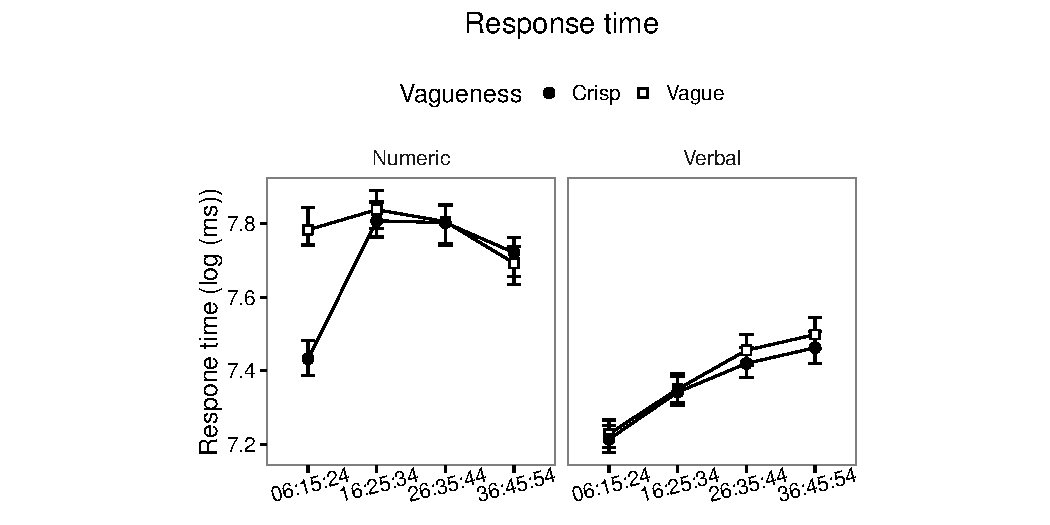
\includegraphics[trim = 20mm 0mm 35mm 0mm, clip, width=.49\textwidth]{images/e2-rtplot-1.pdf}
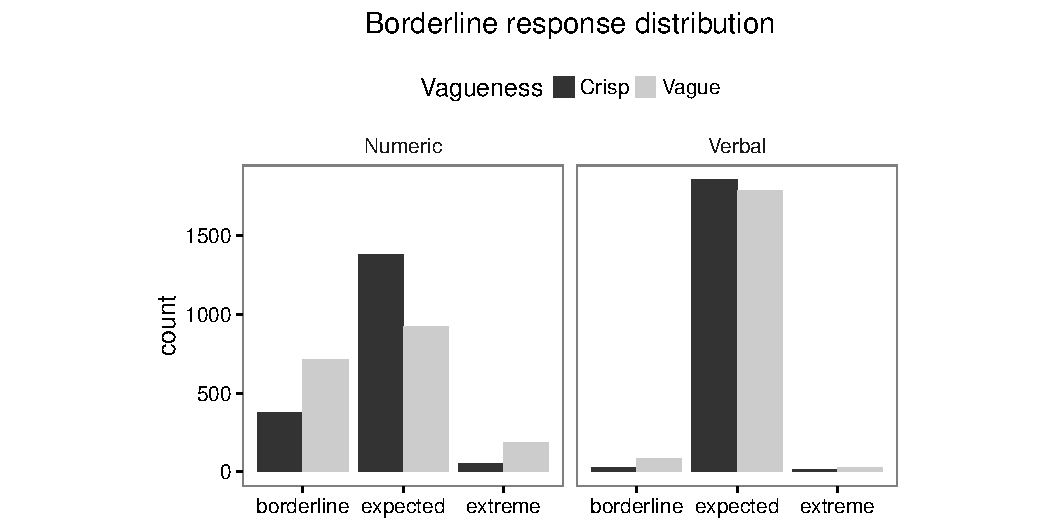
\includegraphics[trim = 20mm 0mm 35mm 0mm, clip, width=.49\textwidth]{images/e2-blBarChart-1}
\caption{Experiment 2 results: mean response times by condition and item, and counts of borderline case responses by condition.}
\label{resultse2}
\end{figure}

\subsection{Discussion} % E2

Experiment 2 tested to see whether when borderline cases are present, vague instructions would speed responses as they did in Experiment 1 when there were no borderline squares. 
We actually found a small (but statistically significant) \emph{disadvantage} of vague instructions: vague instructions slowed people down by 112 ms on average. We also found that the effect of instruction format was significant, with numerical format slowing responses by 689 ms on average, such that the disadvantage of numerical format overwhelmed the contribution of vagueness. The \emph{verbal vague} condition was still responded to faster than the \emph{numerical crisp} condition, so the pattern from Experiment 1 was reproduced, but in the light of the evidence from Experiment 2, in the presence of borderline cases, the advantage that was ascribed to vagueness before now looks more like an advantage of verbal instruction format.

% KvD I've expanded the following:
However, once again there is a possibly confounding factor. Observe that, in Experiment 2, instruction format (i.e., the choice between numeric and verbal) went hand in hand with might be called the (human) {\bf selection algorithm}: To see this, consider the task of selecting the dot array that contains ``few dots": to do this, it suffices to {\em compare} the three arrays and select the one that contains the fewest elements.  To select the dot array that contains "16 dots" seems to require the participant to estimate, and then {\em match}, the cardinality of (at least) one dot array to 16, a process which could plausibly take longer, independently of vagueness. Therefore, our results so far permit the interpretation that what made the instructions in the verbal condition fast is not the fact that they were worded verbally, but that they allowed participants to use a comparison ``algorithm".% (which is known to be faster than matching). % KvD I think we need to say more about this, citing some appropriate papers to support this idea. \textcolor{red}{{\bf--Insert citation}}

In the next two experiments we pitted the comparison algorithm and matching algorithm selection tasks against each other while controlling vagueness and instruction format. In Experiment 3 we restricted all the instructions to \emph{numeric} quantifiers while factorially manipulating vagueness and selection task. In Experiment 4 we ensured that all instructions used \emph{verbal} quantifiers, while also factorially manipulating vagueness and selection task. This allowed us to distinguish between the predictions of the selection task account and the instruction format account. 

%%%%%%%%%%%%%%%%%%%%%%%%
%                            E 3                                     %
%%%%%%%%%%%%%%%%%%%%%%%%

\section{Experiment 3: focus on instructions that contain numerals}

The main aim of Experiment 3 was to see whether vagueness would exert beneficial effects when all conditions used numerals in the instructions, and when there were vague and crisp versions of the instructions for both comparison and matching strategies. The main changes from Experiment 2 were that the human selection task was explicitly controlled (i.e., in whether it amounted to matching or comparison), and that all conditions were constrained to mention a number. We used the same arrays as in Experiment 2. Table \ref{Instructions for e3} shows the instructions for each condition. Note the difference between ``fewer than 20" and ``far fewer than 20": whereas the former cannot have borderline cases (i.e., for each number it is clear whether the number is smaller than 20 or not), the latter can.

%KvD I think we should motivate our choice of materials (especially "far ..er")
%\textcolor{red}{{\bf KvD I think we should motivate our choice of materials (especially "far ..er")}}
% DONE 28 Sept 2017

\begin{table}[htbp]
\centering
\caption{Experiment 3: Instructions arranged by condition for stimuli with $(6,15,24)$ dots and instructions indicating the smaller numbers} 
\label{Instructions for e3}
\begin{tabular}{llll}
instruction				&vagueness			&	selection		&	instruction							\\
format				&					&	task			&									\\
\toprule
\multirow{4}{*}{numeric}	&\multirow{2}{*}{crisp} 	&	matching		& Choose a square with 6 dots 				\\ 
					&					&	comparison 	& Choose a square with fewer than 20 dots 	\\
					\cline{2-4}
					&\multirow{2}{*}{vague} 	&	matching 		& Choose a square with about 10 dots 		\\ 
 					&					&	comparison 	& Choose a square with far fewer than 20 dots 	\\ 
\bottomrule
\end{tabular}
\end{table}%

\subsection{Hypotheses} % E 3
\noindent For Experiment 3, we hypothesised:
{\small
\begin{APAenumerate}
	\item [(H1)] Vague instructions are easier for the reader than crisp ones (main effect of vagueness)
	\item [(H2)] Comparison is easier for the reader than matching (main effect of selection task)
	\item [(H3)] Effects of vagueness are different depending on whether the selection task is matching or comparison (interaction effect selection x vagueness).
\end{APAenumerate}
}

\subsection{Experimental Method} % E 3

38 participants were recruited. We used a 2 x 2 factorial manipulation of vagueness and selection task (see Table \ref{Instructions for e3}).
On each trial an instruction was presented: participants pressed a key to dismiss the instruction, when the dot arrays were presented until the participant responded, and the response time and choice were recorded.

\subsection{Results} % E 3

Response times were trimmed at 2.5 SD separately for each subject, leading to the loss of 204 trials (2.8\% of the trials).
Condition means for the remaining (logged) RTs are plotted in Figure \ref{resultse3}.
A linear mixed model was constructed for the logged response times, 
with sum-coded vagueness, instruction format, (and their interaction), and item as fixed effects, and the same effects as slopes over participant for random effects.

\begin{figure}[htbp]
\centering
\fitfigure{images/e3-rtplot-1.pdf}
%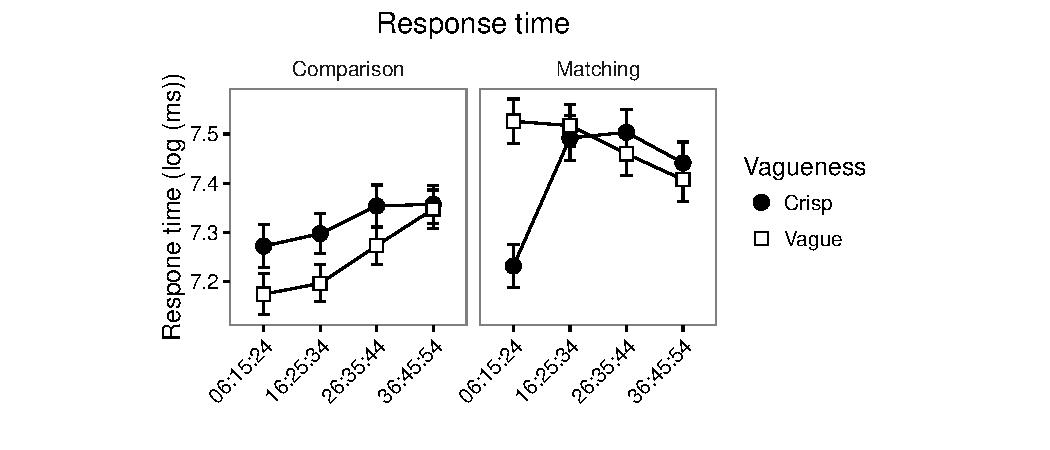
\includegraphics[trim = 20mm 0mm 20mm 0mm, clip, width=.75\textwidth]{images/e3-rtplot-1.pdf}
\caption{Mean response times by condition for Experiment 3 where all instructions were numeric}
\label{resultse3}
\end{figure}

% MG added the values for these stats on 26 Sept 2016
{\small
\begin{APAenumerate}
	\item [(H1)] Vague instructions were non-significantly easier for the reader than crisp instructions when vagueness was considered as a main effect ($\beta=-0.01$, $se=0.01$, $t=-0.4$, $p=0.7158$). 
	\item [(H2)] There was a statistically significant main effect of selection task, with the comparison task speeding responses compared to the matching task ($\beta=0.16$, $se=0.03$, $t=6.2$, $p<0.0001$). 
	\item [(H3)] Vagueness exerted effects in different directions for the comparison task and for the matching task: there was a significant interaction between vagueness and selection task ($\beta=0.13$, $se=0.03$, $t=4.2$, $p<0.0001$). 
Separate analyses were conducted testing for effects of vagueness at each level of the selection task.
Within the comparison task vagueness significantly speeded response times compared with crisp controls ($\beta=-0.07$, $se=0.02$, $t=-3.5$, $p<0.0012$). 
Within the matching task vagueness significantly \emph{slowed} response times compared with crisp controls ($\beta=0.06$, $se=0.02$, $t=2.9$, $p<0.0061$). 
\end{APAenumerate}
}
% MG edited this 27 Sept 2016:
%The cost reduction account was wrong to predict main effect advantages for vagueness, and wrong to predict that vagueness should be beneficial at each level of the selection task: however vagueness was advantageous in the comparison task.
In other words, the cost reduction account was wrong to predict significant main effect advantages for vagueness (although there was a non-significant trend in the \emph{direction} predicted by the cost reduction account), and wrong to predict that vagueness should be beneficial at each level of the selection task: however vagueness was significantly advantageous in the comparison task.


%%%%%%%%%%%%%%%%%%%%%%%%
%                            E 4                                     %
%%%%%%%%%%%%%%%%%%%%%%%%

\section{Experiment 4: focus on instructions that do not contain numerals} % E 4

This experiment mirrors Experiment 3, but focussing on instructions that did not use a number. 
We manipulated vagueness and the selection task (comparison and matching). 
In order to implement the experiment without mentioning numbers in the instructions, we changed the sequence of each trial to include a `target' (i.e., a dot array of a particular cardinality) before the instruction, so that we could then refer back to the target's cardinality in the instruction using expressions like \emph{the same number of dots as the target}; \emph{fewer dots than the target}.
%
This presentation of a target before the main body of the trial shares some features with \citeA[Experiment 2]{Izard20081221}, although in that experiment participants were told the cardinality of the target (called an \emph{inducer} in that paper) whereas in our experiment we did not tell participants the cardinality of the prime array.
An item was thus a combination of a target dot array, an instruction that did not contain a number, and a set of dot arrays taking their cardinalities from the same triples used in Experiment 2.
Table \ref{Instructions for e4} spells out how the instructions were constrained not to mention a numeral and gives examples of targets.

\begin{table}[htp]
\caption{Instructions and targets by condition for Experiment 4}
\begin{center}
\begin{tabular}{llcrl}
Item					&Selection				&Vagueness	&Target	&Choose a square with\ldots						\\
\toprule
\multirow{4}{*}{06:15:24} 	&\multirow{2}{*}{Comparison} 	&Crisp		&20		&\ldots fewer dots than the target					\\
\cline{3-5}
					&						&Vague		&20		&\ldots far fewer dots than the target					\\
					\cline{2-5}
					&\multirow{2}{*}{Matching}		& Crisp		&6		&\ldots the same number of dots as the target			\\
					\cline{3-5}
					& 		 				&Vague		&10 		&\ldots about the same number of dots as the target		\\
					\bottomrule
\end{tabular}
\end{center}
\label{Instructions for e4}
\end{table}%
	
\subsection{Hypotheses}% E 4
\noindent For Experiment 4, we hypothesised:
{\small
\begin{APAenumerate}
	\item [(H1)] Vague instructions are easier for the reader than crisp ones (main effect of vagueness)
	\item [(H2)] Comparison is easier for the reader than matching (main effect of selection)
	\item [(H3)] Effects of vagueness differ depending on whether selection is matching or comparison (interaction effect selection x vagueness, and focussed comparisons at each level of selection).
\end{APAenumerate}
}

\subsection{Results}% E 4
40 volunteers participated.
The results showed that vagueness was beneficial for comparison but detrimental for matching (the same as Experiment 3) even when no numbers were allowed in the instructions. 
Figure \ref{resultse4} shows the means by condition. Our findings were as follows:

% MG added the values for these stats on 27 Sept 2016
{\small
\begin{APAenumerate}
	\item [(H1)] There was no significant main effect of vagueness ($\beta=-0.02$, $se=0.01$, $t=-1.5$, $p=0.1296$). 
	\item [(H2)] There was a main effect of selection, with comparison task instructions leading to faster responses than the matching task instructions ($\beta=0.18$, $se=0.02$, $t=10.4$, $p<0.0001$).  This effect was in the same direction as Experiment 3. 
	\item[(H3)] Vagueness did exert different effects depending on the selection task (main interaction effect of vagueness by selection $\beta=0.12$, $se=0.02$, $t=5.1$, $p<0.0001$). 
Separate analyses of the effect of vagueness were conducted for the comparison task and for the matching task using Bonferroni-adjusted significance thresholds. 
In the comparison task, vagueness resulted in faster response times ($\beta=-0.08$, $se=0.02$, $t=-4.3$, $p<0.0001$). 
In the matching task vagueness slowed response times ($\beta=0.05$, $se=0.01$, $t=3.7$, $p=0.0004$). 
These results are in the same direction as Experiment 3.
\end{APAenumerate}
}

Once again, the cost reduction account was wrong to predict main effect advantages for vagueness, and wrong to predict that vagueness should be beneficial at each level of the selection task: however vagueness was advantageous in the comparison task.

\begin{figure}[htbp]
\centering
\fitfigure{images/e4-rtplot-1.pdf}
\caption{Mean response times by condition for Experiment 4}
\label{resultse4}
\end{figure}

\section{Discussion of experiments 3 and 4}

The main aim of these two experiments was to test whether vagueness confers any cognitive benefits over and above those due to differences in the selection task according to whether the instruction mandates a \emph{comparison} selection task or a \emph{matching} selection task, when number-use is held constant. The main effect of selection task showed that the assumption that the \emph{comparison} task is easier than the \emph{matching} task is well-founded. In both experiments people were reliably quicker to respond in the \emph{comparison} task. 

Vagueness, which was the phenomenon on which our investigation focussed, did not exert a significant main effect in response time. However when the comparison and selection tasks were analysed separately, there was small significant advantage for vagueness in the \emph{comparison} tasks, but a small significant disadvantage for vagueness in the \emph{matching} tasks. 

\section{General Discussion}

To summarise our findings, Experiment 1 showed that responses were faster and more accurate when the instructions were vague than when they were crisp, but the experiment could not distinguish effects of vagueness from those of number-avoidance or selection task: the vague conditions were also in verbal rather than numerical format; and mandated a comparison strategy rather than a matching strategy.  Experiment 2 showed that number avoidance in the verbal format instructions is an important factor driving the faster response times in the task, and that vagueness does not have any additional benefit in either the verbal format instructions or the numerical format instructions. 

However, Experiment 2 did not distinguish benefits of number avoidance from benefits of the comparison selection task. In Experiments 3 and 4 we manipulated vagueness and the selection task, separately at each level of numerical format. Across the two experiments, we found that the comparison-task instructions attracted faster response times than the matching-task instructions. Within the two experiments we found that vagueness exerts benefits when the selection task is \emph{comparison}, but not when the task is \emph{matching}.


\begin{table}[htbp]
\caption{Vagueness as range reduction: a summary of Experiments 3 and 4}
\label{Vagueness as range reduction}
\centering
\begin{tabular}{cccc}
selection task 				& vagueness		& candidates	& effect of vageueness	\\
\toprule
\multirow{ 2}{*}{comparison} 	& crisp 			& 2			& \multirow{ 2}{*}{vagueness advantage}  		\\
\cline{2-3}
  						& vague			& 1			&                                               				\\
\midrule
\multirow{ 2}{*}{matching} 		& crisp 			& 1 			&\multirow{ 2}{*}{vagueness disadvantage}	\\
\cline{2-3}
 						& vague			& 2			&								 	\\
\bottomrule
\end{tabular}
\end{table}

What is one entitled to conclude? Given that we were able to identify a class of situations in which vague expressions led to faster response times than crisp ones, would it be valid to conclude that we have finally discovered an advantage for vagueness that cannot be ascribed to some other factor? We believe the answer to this question is negative. 

To see why, consider Figures \ref{resultse3} and \ref{resultse4}. Both figures depict four conditions, depending on whether the expression was crisp or vague, and depending on whether the referent could be identified using a comparison strategy or not. Two of the resulting four conditions result in an expression that can denote either of two referents; the other two conditions result in an expression that can only denote one referent, with the other possible referent being a marginal candidate at best.

% KvD: I've shortened the text, removing duplication

To see why vagueness has opposite effects, depending on whether it is used in matching or comparison situations, consider the stimulus with (6,15,24) dots. Now compare `Choose a square with 6 dots' with its vague counterpart `Choose a square with about 10 dots': by adding the word `about', we broaden the range of squares that the expression might be referring to. On the other hand, compare `Choose a square with fewer than 20 dots' with `Choose a square with far fewer than 20 dots': by adding the word `far', we did not broaden the range of squares denotable by the expression: we narrow it down, because only some of the squares that have fewer dots may have {\em far} fewer dots.

The benefits of vagueness in the \emph{comparison} task in experiments 3 and 4 could thus be explained as differences in the number of valid targets for the expression. This leads us to speculate that the benefit for vagueness here could be due to the vague expression foregrounding a particular valid target while the crisp expression carries with it the additional task of distinguishing between two alternative valid targets, something we propose to call a ``range-reduction'' benefit.

The observation that conditions with 1 candidate lead to shorter response times than conditions with 2 candidates is consistent with the range reduction hypothesis, but not with the idea that vagueness is beneficial. It appears, in other words, that shorter response times will only result from a vague expression if this expression leads to range reduction. Once again, it is not vagueness itself that has advantages but a phenomenon (namely range reduction) that is an automatic concomitant of vagueness in some types of situations.\\[2ex]
%
\noindent Looking at the entire series of experiments, our findings suggest that the observed benefits of vague expressions in certain situations may be due to factors other than vagueness: factors like avoiding numbers; permitting comparison tasks; and range reduction. The picture that is starting to emerge is subtle: on the one hand, in the situations that we have been studying 
%-- where cooperative speakers refer to an object (e.g., a square) by means of some quantity associated with the object -- 
vagueness is not intrinsically beneficial. On the other hand, vague expressions frequently possess other features that {\em are} beneficial, and these are what give us the incorrect impression that vagueness itself is beneficial. Vagueness may thus have acquired a reputation that it does not deserve. The answer to Lipman's question, of why vagueness permeates human language (see our Introduction), may lie in a different direction after all, possibly relating to benefits for the speaker rather than the hearer. % \cite<see>[chapter 11, for discussion of some possible directions]{vanDeemterBook}.

A comparison may clarify the logic of the situation. In recent years a number of studies, focussing on red wine, have suggested that alcohol, consumed in low doses, may have health benefits. An alternative explanation, however, asserts that it is not the alcohol in the wine that was beneficial, but antioxidants from grapes. If this alternative explanation is correct, then alcohol may not be healthy after all.\\[2ex]
%
{\bf Implications for NLG systems.} Our findings suggest a re-think of the questions on which much research on the utility of vagueness rests. The question of how a particular piece of quantitative information is best conveyed through language is an important one for practical NLG; years of research on the logic of vagueness -- giving rise to such techniques as Partial Logic \cite<e.g.,>{Fine}, Probabilistic Logic \cite{Edgington}, and Fuzzy Logic \cite{Zadeh} -- have primed the research community to expect that the utility of vagueness is an important part of the answer, but our findings call this expectation into question. 

Although our own studies in this article have focussed on vagueness in descriptive Noun Phrases, it seems plausible that vagueness plays a similar role in other linguistic constructs. For example, consider reports on air temperature (cf., our discussion of NLG at the start of the paper). Given a temperature measurement or prediction as input, an NLG system might say that it will be
%
\begin{quote}
(a) {\em 27.2 degrees Celsius}, or\\
(b) {\em approximately 27 degrees}, or\\
(c) {\em above 25 degrees}, or\\
(d) {\em warm}, 
\end{quote}
%
among other candidate expressions. If the linguistic literature is to be believed, then options (a) and (c) convey crisp information, whereas (b) and (d) are vague (i.e., they permit borderline cases). From our own experiments and the ones discussed in section 1, there is no evidence that  vagueness should be beneficial for hearers. Rather than asking whether a candidate expression is vague, other questions might shed more light on the NLG system's choice, similar to the ones identified in our studies. These questions might focus on the amount of information that a given expression conveys (i.e., on granularity), on the avoidance of numbers, and on the use of evaluative terms. Let's see how this might pan out for the examples at hand.

First, the experiments by \citeauthor{Mishra01042011} suggest that it is important how much information is conveyed by an expression, and their findings are echoed by our own thoughts about range reduction (following Experiments 3 and 4). In the case of (a)--(d) above, it appears that (a) conveys the most detailed information (designating the smallest segment of the temperature scale), followed by (b), then (d), then (c) (e.g., 40 degrees is above 25, but at 40 Celsius the word ``warm" is likely to give way to ``hot" or ``scorching"): 
%
\begin{quote}
$a < b < d < c$
\end{quote}
%
If these hunches are correct then an {\em expert} may  to prefer expression (a), because it gives her the most detailed information on which to base her decisions. On the other hand, expression (d) (``warm") is shorter than the other three and avoids the use of numbers; our experiments suggest that this may make (d) more rapidly understood than its competitors; earlier experiments point in the same direction, given the evaluative nature of ``warm" (see our section 1 and  \citeA{peters2009bringing}), which is especially important if the hearer is unfamiliar with the metric used (e.g., because she is more used to Fahrenheit). These considerations suggest that {\em non-experts} might prefer expression (d). If results of this kind were to be confirmed by experiments, they would be applicable in practical NLG, though care would need to be exercised to take the purpose of the communication into account.\footnote{One reason why ``warm" might be less preferred than these considerations suggest is that, in the weather context, some very frequently occurring numbers, such as 20 (degrees), could be relatively easy to process, analogous to the subitizable numbers of \protect\citeA{trick1994small}, see our section \ref{method}. Note that in the experiments reported in this paper, the purpose of the utterances investigated was always clear (e.g., instructing people on a weight loss program \cite{Mishra01042011}; informing a patient's choice of hospital \cite{peters2009bringing}; or selecting a dot array (in our own studies).} 

One way to see why vagueness (as defined in our Introduction) may not matter much for NLG -- and for human communication -- is the following thought experiment. Suppose a group of speakers understand the word ``warm" as vague, agreeing that temperatures above 26 count as warm, and temperatures below 24 do not count as warm, but considering temperatures between 24 and 26 as borderline cases. Now one day these speakers agree to sharpen up their definition deciding that, henceforth, ``warm" means ``$>25$ degrees" (as in (c) above): this decision resolves the borderline cases, while everything else remains the same. It seems unlikely that this change in language use, from a vague meaning to a crisp one (i.e., one that has no borderline cases anymore), would lower the utility of the word. Our experimental findings are consistent with this idea.

% KvD Bracketed out the following for now:
%A more radical perspective on our findings might say that the distinction between crisp and vague expressions, which is taken for granted in the bulk of the linguistic literature, is mistaken, because expressions such as ``above 25 degrees" (and ``fewer than 20 dots") are not equally felicitous in all situations in which they can be truthfully applied. For example, when the temperature is 40 degrees, then a weather report saying that it is ``above 25 degrees" would be correct yet misleading: this description might be felicitous as a description of temperatures between (roughly) 26-28 degrees, borderline felicitous for 29-33 degrees, and infelicitous at even higher temperatures. At its most bold, this perspective would assert that the applicability of {\em every} linguistic expression has borderline cases, hence Lipman's question (see section 1) does not arise. This radical perspective -- which would have drastic implications for the construction of an NLG system -- can only be indicated here, but not discussed at length.

\setcounter{secnumdepth}{0}
\bibliography{v-special-issue-2016}
\end{document}
